\subsection{Points-to Analyse}
\label{subsec:pointsto}

Die Points-To Analysis (dt. Pointer-Analyse) ist eine Technik zur Berechnung der Menge von Objekten bzw. dessen Speicherbereichen, auf die eine Programm Variable zur Laufzeit zeigen kann\parencite{Hind2001, Smaragdakis2015}. 
Da der komplette Quellcode des zu analysierenden Programmes vorliegen muss, ist die Pointer-Analyse eine statische Analysetechnik.

Die Pointer Analyse startet mit allen Eingangspunkten, beispielsweise der main()-Methode. Dann werden iterativ alle erreichbaren Methoden verarbeitet, bis ein Fixpunkt erreicht ist. 
Der Java-Bytecode wird durch das Frontend des Compilers\footnote{das Frontend ist eine von 3 Stufen des Kompilierungsvorganges (Front end, Middle end, Back end), auch Analysephase genannt. Dabei wird der Code analyisiert, strukturiert und auf Fehler geprüft.} in eine Zwischenform 
überführt (engl. intermediate representation = IR), die das Programm repräsentiert und weitere Optimierungen und Transformationen ermöglicht\parencite{Simon2015}. Diese Zwischenform wird als nächstes in einen 
sog. \textit{type-flow graph} konvertiert. Jeder Knoten stellt eine Operation auf einem Objekttypen dar. Die gerichteten Kanten verlaufen von der Definition des Objektes bis zur tatsächlichen Verwendung. 
Jeder Knoten verwaltet eine Liste mit Typen (engl. \textit{type state}), die diesen Knoten erreichen können (siehe Abbildung~\ref{fig:typeflowgraph}). Die Listen werden durch die Kanten des Graphen propagiert. Sobald einer Liste Typen hinzugefügt werden, wird die Änderung an alle weiteren Verwendungen (Kindelemente eines Knotens) propagiert. Typlisten dürfen nur Elemente hinzugefügt werden, und keine Elemente gelöscht werden, damit sichergestellt ist das die Analyse den Fixpunkt erreicht und terminiert. Für jeden Typ, schaut die Pointer Analyse ob  dieser instanziiert ist. Falls dem so ist, wird er 
 durch Bytecodes markiert. Für jedes Feld, wird separat ermittelt ob die Felder während der Laufzeit nur gelesen oder auch geschrieben werden\parencite{Wimmer2019}, und als \textit{write} oder {read} markiert. Felder die als \textit{read} markiert sind, werden bereits während der Ahead-of-time Kompilierung berechnet, statt erst zur Laufzeit (sog. \textit{constant-folding}, \parencite[Kapitel 4.2]{Grumberg2014}).

\begin{figure}[!ht]
%figure full paperwidth and trim the left and right empty space from it
   \makebox[\textwidth]{
     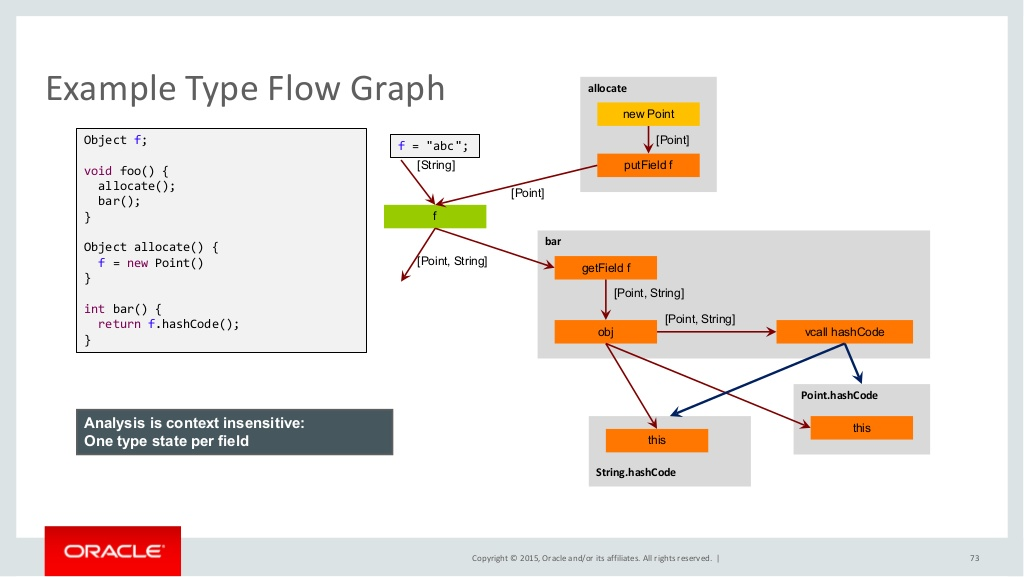
\includegraphics[trim = 8mm 0mm 16mm 0mm,width=1.1\paperwidth]{resources/graal-tutorial-at-cgo-2015.jpg}
   }
\caption{Type-flow Graph, \parencite[Folie 71 \& 72]{Wimmer2015}}
	\label{fig:typeflowgraph}
\end{figure}
